\chapter{Aufbau}
\section{Übersicht des Experimentierplatzes}

\begin{figure}[htbp]
    \centering
    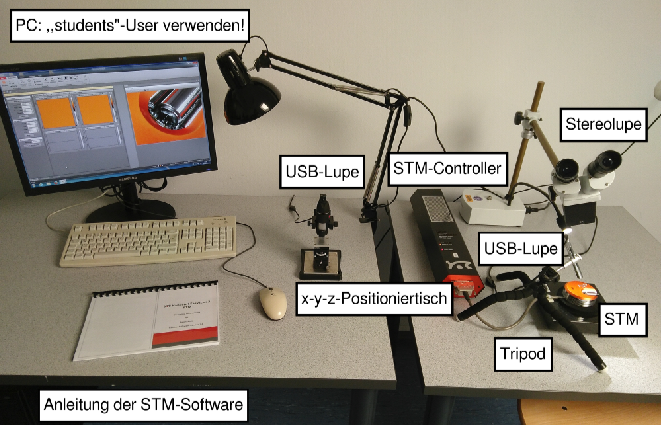
\includegraphics[width=0.75\textwidth]{figs/Versuchsaufbau1.png}
    \caption{Experimentelle Station für das P422-Rastertunnelmikroskopie-Experiment. \cite{praktikum}}
    \label{fig:Versuchaufbau1}    
\end{figure}
Der in Abbildung \ref{fig:Versuchaufbau1} dargestellte Versuchsaufbau wird für die Durchführung des Experiments verwendet. Zentrales Messinstrument ist ein Rastertunnelmikroskop (RTM Abbildung \ref{fig:RTM}). Das verwendete RTM verfügt über einen integrierten Controller und wird mit der Software „NaioSTM“ betrieben.

Eine USB-Lupe oberhalb des x-y-z-Positioniertisches ermöglicht die Erfassung und Qualitätskontrolle von Proben und Spitzen vor und nach Messungen mit dem RTM. Das zu untersuchende Objekt wird durch einen am Positioniertisch befestigten Magneten fixiert. Die Bilder der USB-Lupe werden mit der Software „amcap“ erstellt. Eine zweite USB-Lupe ist oberhalb des RTM angebracht und dient der Beobachtung der sich der Spitze nähernden Probe. Diese Lupe ist auf einem Stativ montiert und wird über die RTM-Software gesteuert.

Die Eingabegeräte und der zugehörige Computer sind auf zwei separaten Tischen platziert, um Vibrationen durch manuelle Bedienung zu reduzieren und so Störungen der Messergebnisse zu minimieren. Das RTM ist zusätzlich auf einem vibrationsdämpfenden Rahmen montiert, um zusätzliche Störungen zu reduzieren.
\begin{figure}
    \centering
    \includegraphics[width=0.75\textwidth]{figs/Versuch_box}
    \caption{Weitere Materialien für den Aufbau. \cite{praktikum}}
    \label{fig:Versuch box}
\end{figure}
 Alle Proben, Pinzetten, der Probenbehälter und weitere Materialien befinden sich in der in Abbildung \ref{fig:Versuch box} dargestellten Box. Für die HOPG-Probe wird eine flache Pinzette verwendet, für die übrigen Proben eine Spezialpinzette. Die Box enthält außerdem zusätzliches Material zur Reinigung und Handhabung der Proben. Die Proben und Spitzen werden in die entsprechenden Halterungen des STM eingesetzt, und die Schutzkappe des STM-Anschlusses wird für das Experiment entfernt.

\section{Das Rastertunnelmikroskop (RTM): Aufbau und Funktionsweise}

\subsubsection{Aufbau}

\begin{figure}[H]
\centering
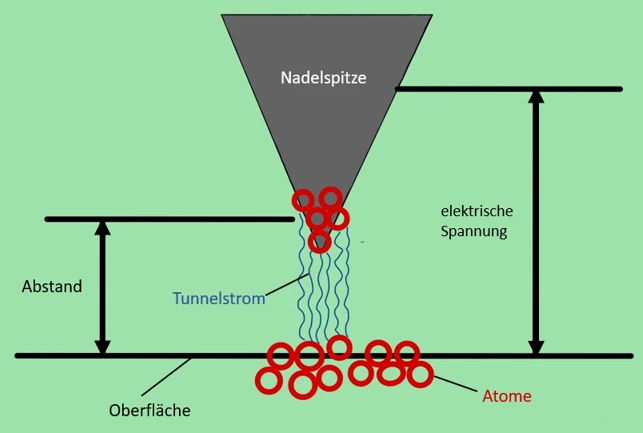
\includegraphics[width=0.75\textwidth]{figs/RTM}
\caption{Aufbau des RTM \cite{RTM}}
\label{fig:RTM}
\end{figure}

Das Rastertunnelmikroskop (RTM, engl. STM für Scanning Tunneling Microscope), wie in Abbildung \ref{fig:RTM} dargestellt, ist ein hochauflösendes Analyseinstrument zur Darstellung leitfähiger Oberflächen im atomaren Maßstab.
\begin{figure}[H]
\centering
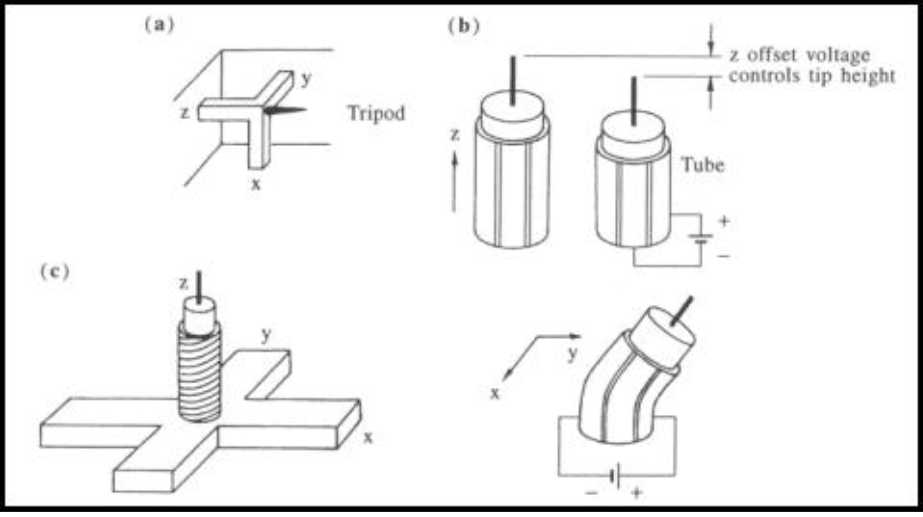
\includegraphics[width=0.75\textwidth]{figs/RTM piezo}
\caption{a)Schematischer Aufbau der piezoelektrischen Stellglieder, b)Aufbau vom "Single Tube Scanner", c)Piezokreuz mit aufgesetztem "Single Tube" \cite{piezo}}
\label{fig:piezo}
\end{figure}
Das STM (Abbildung \ref{fig:piezo}) nutzt piezoelektrische Stellglieder zur präzisen Positionierung der Spitze in drei Raumrichtungen. Der dazu entstehende Piezoeffekt beschreibt die Eigenschaft bestimmter Kristalle, sich unter elektrischer Spannung mechanisch zu verformen, in diesem Fall im Sub-Nanometerbereich. Dadurch kann die Spitze rasterartig über die Probe bewegt und gleichzeitig der Abstand hochpräzise geregelt werden. Der Tunnelstrom wird über einen Strom-Spannungswandler detektiert und in einem PID-Regelkreis (Propotional, Integral and Differential) verarbeitet, der die z-Position der Spitze so anpasst, dass der Strom konstant bleibt (''Constant Current Mode''). Die Spannung am z-Piezo ist damit direkt proportional zur Oberflächenhöhe. Alternativ kann im ''Constant Height Mode'' gearbeitet werden, bei dem der Tunnelstrom selbst das Bild liefert, während die Höhe konstant bleibt. Dieser Modus ist schneller, aber risikobehafteter bei rauen Oberflächen.


\subsubsection{Funktionsweise}
Es wurde Anfang der 1980er Jahre von Gerd Binnig und Heinrich Rohrer entwickelt und basiert auf einem fundamentalen quantenmechanischen Phänomen: dem Tunneleffekt.

\paragraph{Tunneleffekt}
\begin{figure}[H]
\centering
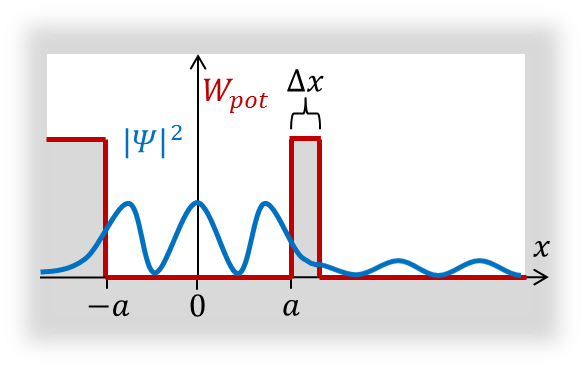
\includegraphics[width=0.75\textwidth]{tunneff.png}
\caption{Veranschaulichung des Tunneleffekts:
$\psi$ entspricht der Wellenfunktion des Teilchens, welche das quantenmechanische Verhalten des Teilchens beschreibt, $W_{pot}$ gibt die Höhe der Potentialbarriere (grau) an. \cite{Tunneleff}}
\label{fig:tunnel}  
\end{figure}
Dieser Tunneleffekt, wie in \cref{fig:tunnel} illustriert, beschreibt die Möglichkeit von Teilchen, eine Energiebarriere zu durchqueren, obwohl ihre Energie unterhalb der Höhe dieser Barriere liegt. 
Dies ist ein Verhalten, das aus klassischer Sicht unmöglich wäre. In der Quantenmechanik wird ein Elektron durch eine Wahrscheinlichkeitsverteilung beschrieben, und seine Aufenthaltswahrscheinlichkeit reicht über potenzielle Barrieren hinaus.\\
\begin{figure}[H]
\centering
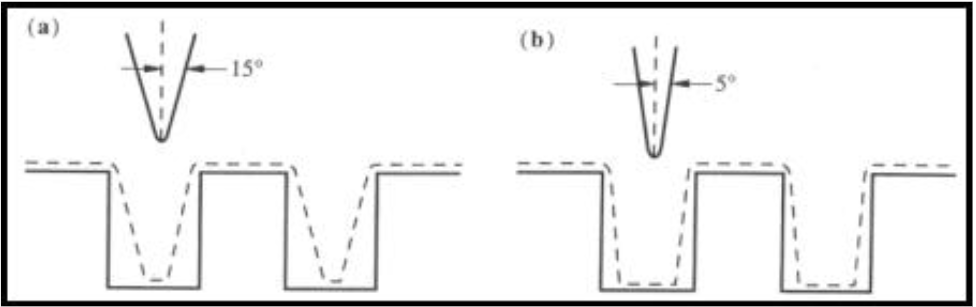
\includegraphics[width=0.75\textwidth]{figs/tunnelspitze}
\caption{ Rasterverlauf der Spitze für a)einen kleinen Konuswinkel b)einen großen Konuswinkel \cite{piezo}}
\label{fig:raster}
\end{figure} 



Wenn sich eine scharf zugespitzte metallische Spitze (in diesem Fall Platinum-Iridium (Pt-Ir)) einer leitfähigen Oberfläche bis auf wenige Ångström nähert (Abbildung \ref{fig:raster}) und eine geringe Spannung anliegt, besteht eine endliche Wahrscheinlichkeit, dass Elektronen von der Spitze zur Probe oder umgekehrt tunneln. Dieser Tunnelstrom ist extrem empfindlich gegenüber dem Abstand, den er sinkt exponentiell mit wachsender Distanz (d). 
Daraus ergibt sich die Möglichkeit, atomare Höhenunterschiede auf der Oberfläche zu detektieren.

%Weitere zentrale Begriffe für das Verständnis des STM sind die Austrittsarbeit, jene Mindestenergie, die nötig ist, um ein Elektron aus einem Festkörper ins Vakuum zu bringen, sowie das Ferminiveau, das die höchste besetzte Energieniveaulinie bei absolutem Nullpunkt darstellt. Der Tunnelstrom 
%\begin{equation}
%    T \propto e^{-2\kappa d}, \quad \text{mit } \kappa = \sqrt{\frac{2m(\Phi - E)}{\hbar^2}}
%\end{equation}
%\cite{Temperatur}
%hängt unter anderem von der Differenz der Ferminiveaus von Spitze und Probe sowie von deren jeweiligen Austrittsarbeiten ab.

\paragraph{Funktionsweise des PID-Reglers}

Ein PID-Regler (Proportional-Integral-Differential-Regler) wird im Rastertunnelmikroskop (RTM) verwendet, um die Höhe der Spitze über der Probe so zu steuern, dass der Tunnelstrom konstant bleibt. Der Regler besteht aus drei Komponenten:


\begin{itemize}
    \item \textbf{Proportionalanteil (P)}: Reagiert direkt auf die Abweichung des gemessenen Tunnelstroms $I_t$ vom Sollwert $I_{t, \text{Soll}}$ und passt die Spitze entsprechend an.
    \item \textbf{Integralanteil (I)}: Berücksichtigt vergangene Abweichungen und sorgt für eine langfristige Stabilisierung.
    \item \textbf{Differentialanteil (D)}: Reagiert auf schnelle Änderungen und verhindert Überschwingungen.
\end{itemize}

Die Regelfunktion ist gegeben durch:

\begin{equation}
    u(t) = K_p e(t) + K_i \int_0^t e(\tau) d\tau + K_d \frac{d e(t)}{dt},
\end{equation}

wobei $e(t) = I_{t, \text{Soll}} - I_t$ die Regelabweichung ist und die Verstärkungsfaktoren $K_p$, $K_i$ und $K_d$ das Regelverhalten bestimmen.

\paragraph{Strom-Spannungs-Wandler}
In einem Rastertunnelmikroskop (RTM) wandelt ein Spannungs-Strom-Wandler eine angelegte Spannung in einen präzisen Tunnelstrom um. Dieser Strom hängt exponentiell vom Abstand zwischen Spitze und Probe ab \cite{Tunnelstrom}:
\begin{equation}
    I \propto e^{-\alpha d}, \quad \text{mit } \kappa \approx 1\, \text{\AA}^{-1}.
\end{equation}


Ein Transimpedanzverstärker misst und wandelt den Strom um, sodass ein PID-Regler die Spitze in Echtzeit verfolgen und einen konstanten Strom aufrechterhalten kann. Diese Regelung ist unerlässlich, da sie dem RTM ermöglicht, atomare Auflösung zu erreichen und feine Oberflächenstrukturen abzubilden.

\paragraph{Betriebsmodi des Rastertunnelmikroskops}

Die Höhenunterschiede der Probe können durch unterschiedliche Betriebsmodi des RTM erfasst werden. Im \textbf{''Constant Current Mode''} wird die Spitze so positioniert, dass der Tunnelstrom konstant bleibt. Dies geschieht durch Anpassung der z-Position der Spitze mittels eines PID-Regelkreises, der die Höhe der Spitze in Abhängigkeit vom gemessenen Tunnelstrom regelt. Im \textbf{''Constant Height Mode''} hingegen wird die z-Position der Spitze konstant gehalten, und der Tunnelstrom variiert entsprechend den Höhenunterschieden der Probe. Dieser Modus ist schneller, birgt jedoch das Risiko, dass die Spitze bei größeren Höhenunterschieden die Probe berührt und beschädigt.

\chapter{Übersicht des Versuchsablaufs}


Es kommen zwei Varianten des STM zum Einsatz: eines mit externem Controller und Easyscan-Software, das andere mit integriertem Controller und NaioSTM-System. Beide Systeme beinhalten ein STM-Gerät, eine Probenhalterung mit Magnetfixierung, eine USB-Lupe zur optischen Kontrolle sowie eine stereoskopische Beobachtungseinheit. Das Gerät wird über einen Computer angesteuert, der auch die Datenaufnahme und Visualisierung übernimmt.

Die STM-Spitze wird durch kontrolliertes Abreißen eines Pt-Ir-Drahts hergestellt und mit einer Halterung in das Gerät eingesetzt. Zur Dokumentation werden sowohl Spitze als auch Probe mit einer USB-Lupe mikroskopiert und kalibriert. Vor Messbeginn wird die Spitze durch mechanisches Advance der Probe angenähert, gefolgt von einem automatisierten Approach, bei dem der Tunnelkontakt präzise erkannt wird.
Die Durchführung des Experiments erfolgt in mehreren Schritten, die im Folgenden detailliert beschrieben werden. Zunächst wird die STM-Spitze vorbereitet und kalibriert, gefolgt von der Probenvorbereitung und der eigentlichen Messung.

Die erste Messungen erfolgt stets im ''Constant Current Mode'', um Schäden an der Spitze durch unkontrollierte Höhenunterschiede zu vermeiden. Typische Startparameter sind eine Tunnelspannung von $U = 1\,\text{V}$ und ein Strom von $I = 1\,\text{nA}$. Die PID-Regelparameter ($P = 1000$, $I = 2000$, $D = 0$) gewährleisten eine stabile Annäherung und Nachführung. Mit der Software wird ein Bildbereich (z.\,B. $200\,\text{nm} \times 200\,\text{nm}$) definiert und gescannt. Die resultierenden Bilder zeigen die topografischen Eigenschaften der Gold-Proben mit hoher lateraler und vertikaler Auflösung.

Zur Analyse von HOPG-Proben wird die Graphitoberfläche zunächst mit Tesafilm abgezogen, um eine frische Schicht freizulegen. Nach dem Einbau wird ein Grobscan durchgeführt. Bei Erfolg werden schrittweise kleinere Bildbereiche gewählt ($10\,\text{nm} \times 10\,\text{nm}$ bis hin zu $4\,\text{nm} \times 4\,\text{nm}$), um atomare Strukturen zu erkennen. Dabei sollten die hexagonale Gitterstruktur von Graphit sichtbar sein. Mit geeigneter Software lassen sich Gitterabstände und -winkel bestimmen, um die Kalibrierung des STM zu überprüfen. Bei Problemen mit der Auflösung helfen Methoden wie Parameteranpassung, Spannungspulse zur Reinigung der Spitze oder der Austausch der Spitze.

Während des gesamten Versuchs werden alle relevanten Messparameter dokumentiert, einschließlich Rastergeschwindigkeit, Spannungs- und Stromwerte, PID-Einstellungen und verwendete Spitze. Die Bilder werden zur Auswertung exportiert und analysiert.
